% answers.tex —— 2004 年·全国卷Ⅳ·理科 · 参考答案与详细解析片段
% 由 tools/generate_projects.py 依来源总账自 2004/2004_数学真题_全国4理_试题.md + 2004/2004_数学真题_全国4理_解析正文.md + 2004/2004_数学真题_全国4理_答案要点.md 生成，勿手改（改源 MD 后重跑）


\begin{gktip}
固定源 PDF 为印刷页码 194–195 的两页题面，不附答案。以下解析均依据固定源独立推导复算；第 20 题图形在 LaTeX 工程中以 TikZ/PGFPlots 矢量源重绘。
\end{gktip}

\begin{answer}
\gksolhead{1}{}

\textbf{题目}：

已知集合 $M=\{0,1,2\}$，$N=\{x\mid x=2a,a\in M\}$，则集合 $M\cap N=$\mbox{（　　）}

（A）$\{0\}$　　（B）$\{0,1\}$　　（C）$\{1,2\}$　　（D）$\{0,2\}$

\Needspace{4\baselineskip}
\textbf{解析}

已知集合 $M=\{0,1,2\}$。
\Needspace{5\baselineskip}
根据集合 $N$ 的定义：
\nopagebreak[4]
\[
N=\{x\mid x=2a,a\in M\}=\{2\times 0,2\times 1,2\times 2\}=\{0,2,4\}.
\]
\Needspace{5\baselineskip}
求集合 $M$ 与 $N$ 的交集：
\nopagebreak[4]
\[
M\cap N=\{0,1,2\}\cap\{0,2,4\}=\{0,2\}.
\]
故选 D。

\gkanswer{答案：D}

\end{answer}
\begin{answer}
\gksolhead{2}{}

\textbf{题目}：

函数 $y=\mathrm{e}^{2x}$（$x\in\mathbf{R}$）的反函数为\mbox{（　　）}

（A）$y=2\ln x$（$x>0$）　　（B）$y=\ln(2x)$（$x>0$）

（C）$y=\dfrac{1}{2}\ln x$（$x>0$）　　（D）$y=\dfrac{1}{2}\ln 2x$（$x>0$）

\Needspace{4\baselineskip}
\textbf{解析}

由 $y=\mathrm{e}^{2x}$（$x\in\mathbf{R}$），
因为指数函数 $\mathrm{e}^{2x}>0$，所以函数的值域为 $(0,+\infty)$，即 $y>0$。
\Needspace{5\baselineskip}
方程两边取以 $\mathrm{e}$ 为底的自然对数得：
\nopagebreak[4]
\[
2x=\ln y\implies x=\frac{1}{2}\ln y.
\]
\Needspace{5\baselineskip}
习惯上互换自变量与因变量字母 $x,y$，得反函数为：
\nopagebreak[4]
\[
y=\frac{1}{2}\ln x\quad (x>0).
\]
故选 C。

\gkanswer{答案：C}

\end{answer}
\begin{answer}
\gksolhead{3}{}

\textbf{题目}：

过点 $(-1,3)$ 且垂直于直线 $x-2y+3=0$ 的直线方程为\mbox{（　　）}

（A）$2x+y-1=0$　　（B）$2x+y-5=0$

（C）$x+2y-5=0$　　（D）$x-2y+7=0$

\Needspace{4\baselineskip}
\textbf{解析}

已知直线 $x-2y+3=0$ 的斜率为 $k_0=\dfrac{1}{2}$。
\Needspace{5\baselineskip}
因为所求直线与该直线垂直，所以所求直线的斜率 $k$ 满足：
\nopagebreak[4]
\[
k\cdot k_0=-1\implies k=-\frac{1}{k_0}=-2.
\]
\Needspace{5\baselineskip}
又所求直线经过点 $(-1,3)$，由直线的点斜式方程得：
\nopagebreak[4]
\[
y-3=-2(x-(-1))\implies y-3=-2x-2.
\]
\Needspace{5\baselineskip}
移项整理得：
\nopagebreak[4]
\[
2x+y-1=0.
\]
故选 A。

\gkanswer{答案：A}

\end{answer}
\begin{answer}
\gksolhead{4}{}

\textbf{题目}：

$\left(\dfrac{1-\sqrt{3}\mathrm{i}}{1+\mathrm{i}}\right)^2=$\mbox{（　　）}

（A）$\sqrt{3}+\mathrm{i}$　　（B）$-\sqrt{3}-\mathrm{i}$　　（C）$\sqrt{3}-\mathrm{i}$　　（D）$-\sqrt{3}+\mathrm{i}$

\Needspace{4\baselineskip}
\textbf{解析}

\Needspace{5\baselineskip}
计算复数表达式：
\nopagebreak[4]
\[
\left(\frac{1-\sqrt{3}\mathrm{i}}{1+\mathrm{i}}\right)^2=\frac{(1-\sqrt{3}\mathrm{i})^2}{(1+\mathrm{i})^2}.
\]
\Needspace{5\baselineskip}
分别计算分子和分母：
\nopagebreak[4]
\[
(1-\sqrt{3}\mathrm{i})^2=1-2\sqrt{3}\mathrm{i}+(\sqrt{3}\mathrm{i})^2=1-2\sqrt{3}\mathrm{i}-3=-2-2\sqrt{3}\mathrm{i},
\]
\nopagebreak[4]
\[
(1+\mathrm{i})^2=1+2\mathrm{i}+\mathrm{i}^2=1+2\mathrm{i}-1=2\mathrm{i}.
\]
\Needspace{5\baselineskip}
代入分式中化简：
\nopagebreak[4]
\[
\frac{-2-2\sqrt{3}\mathrm{i}}{2\mathrm{i}}=\frac{-1-\sqrt{3}\mathrm{i}}{\mathrm{i}}=\frac{(-1-\sqrt{3}\mathrm{i})(-\mathrm{i})}{-\mathrm{i}^2}=\frac{\mathrm{i}+\sqrt{3}\mathrm{i}^2}{1}=\mathrm{i}-\sqrt{3}=-\sqrt{3}+\mathrm{i}.
\]
故选 D。

\gkanswer{答案：D}

\end{answer}
\begin{answer}
\gksolhead{5}{}

\textbf{题目}：

不等式 $\dfrac{x(x+2)}{x-3}<0$ 的解集为\mbox{（　　）}

（A）$\{x\mid x<-2\text{ \text{或} }0<x<3\}$　　（B）$\{x\mid -2<x<2\text{ \text{或} }x>3\}$

（C）$\{x\mid x<-2\text{ \text{或} }x>0\}$　　（D）$\{x\mid x<0\text{ \text{或} }x<3\}$

\Needspace{4\baselineskip}
\textbf{解析}

解不等式 $\dfrac{x(x+2)}{x-3}<0$。
\Needspace{5\baselineskip}
该分式不等式等价于：
\nopagebreak[4]
\[
x(x+2)(x-3)<0.
\]
方程 $x(x+2)(x-3)=0$ 的三个实数根分别为 $-2,0,3$。
利用数轴标根法（穿针引线法）：
\begin{itemize}
\item 当 $x>3$ 时，三因式均为正，积为正；
\item 当 $0<x<3$ 时，积为负；
\item 当 $-2<x<0$ 时，积为正；
\item 当 $x<-2$ 时，三因式均为负，积为负。
\end{itemize}
\Needspace{5\baselineskip}
因此，使积小于 0 的解集为：
\nopagebreak[4]
\[
\{x\mid x<-2\text{ \text{或} }0<x<3\}.
\]
故选 A。

\gkanswer{答案：A}

\end{answer}
\begin{answer}
\gksolhead{6}{}

\textbf{题目}：

等差数列 $\{a_n\}$ 中，$a_1+a_2+a_3=-24$，$a_{18}+a_{19}+a_{20}=78$，则此数列前 20 项和等于\mbox{（　　）}

（A）160　　（B）180　　（C）200　　（D）220

\Needspace{4\baselineskip}
\textbf{解析}

\Needspace{5\baselineskip}
在等差数列 $\{a_n\}$ 中，由等差数列的性质：
\nopagebreak[4]
\[
(a_1+a_2+a_3)+(a_{18}+a_{19}+a_{20})=(a_1+a_{20})+(a_2+a_{19})+(a_3+a_{18})=3(a_1+a_{20}).
\]
已知 $a_1+a_2+a_3=-24$，$a_{18}+a_{19}+a_{20}=78$，
\Needspace{5\baselineskip}
两式相加得：
\nopagebreak[4]
\[
3(a_1+a_{20})=-24+78=54\implies a_1+a_{20}=18.
\]
\Needspace{5\baselineskip}
前 20 项和公式为：
\nopagebreak[4]
\[
S_{20}=\frac{20(a_1+a_{20})}{2}=10(a_1+a_{20})=10\times 18=180.
\]
故选 B。

\gkanswer{答案：B}

\end{answer}
\begin{answer}
\gksolhead{7}{}

\textbf{题目}：

对于直线 $m$、$n$ 和平面 $\alpha$，下面命题中的真命题是\mbox{（　　）}

（A）如果 $m\subset\alpha$，$n\not\subset\alpha$，$m$、$n$ 是异面直线，那么 $n\parallel\alpha$

（B）如果 $m\subset\alpha$，$n\not\subset\alpha$，$m$、$n$ 是异面直线，那么 $n$ 与 $\alpha$ 相交

（C）如果 $m\subset\alpha$，$n\parallel\alpha$，$m$、$n$ 共面，那么 $m\parallel n$

（D）如果 $m\parallel\alpha$，$n\parallel\alpha$，$m$、$n$ 共面，那么 $m\parallel n$

\Needspace{4\baselineskip}
\textbf{解析}

逐项分析各命题的真伪：
\begin{itemize}
\item 对于（A）：如果 $m\subset\alpha$，$n\not\subset\alpha$，$m\text{、}n$ 是异面直线，直线 $n$ 既可能平行于平面 $\alpha$，也可能与平面 $\alpha$ 相交（只要交点不落在直线 $m$ 上），故（A）为假命题；
\item 对于（B）：同理，$n$ 可以平行于平面 $\alpha$（在平面外作一条与 $m$ 异面的平行线即可），不一定相交，故（B）为假命题；
\item 对于（C）：已知 $m\subset\alpha$，$n\parallel\alpha$。因为 $m\text{、}n$ 共面，设它们所确定的平面为 $\beta$。则平面 $\beta$ 经过直线 $n$ 且与平面 $\alpha$ 相交于直线 $m$。由线面平行的性质定理可知，如果一条直线平行于一个平面，经过这条直线的平面和这个平面相交，那么这条直线就和交线平行，因此必有 $m\parallel n$。故（C）为真命题；
\item 对于（D）：平行于同一个平面的两条共面直线，在它们所在的平面内完全可以相交，故（D）为假命题。
\end{itemize}
综上，真命题是（C）。
故选 C。

\gkanswer{答案：C}

\end{answer}
\begin{answer}
\gksolhead{8}{}

\textbf{题目}：

已知椭圆的中心在原点，离心率 $e=\dfrac{1}{2}$，且它的一个焦点与抛物线 $y^2=-4x$ 的焦点重合，则此椭圆方程为\mbox{（　　）}

（A）$\dfrac{x^2}{4}+\dfrac{y^2}{3}=1$　　（B）$\dfrac{x^2}{8}+\dfrac{y^2}{6}=1$

（C）$\dfrac{x^2}{2}+y^2=1$　　（D）$\dfrac{x^2}{4}+y^2=1$

\Needspace{4\baselineskip}
\textbf{解析}

已知抛物线方程为 $y^2=-4x$。
对比标准形式 $y^2=-2px$ 得 $2p=4\implies p=2$，其焦点在 $x$ 轴负半轴上，焦点坐标为 $\left(-\dfrac{p}{2},0\right)=(-1,0)$。
因为椭圆的中心在原点，且它的一个焦点与抛物线的焦点重合，
所以椭圆的焦点在 $x$ 轴上，焦点坐标为 $(\pm 1,0)$，即半焦距 $c=1$。
又已知椭圆离心率 $e=\dfrac{c}{a}=\dfrac{1}{2}$，
\Needspace{5\baselineskip}
所以长半轴长为：
\nopagebreak[4]
\[
a=\frac{c}{e}=\frac{1}{1/2}=2\implies a^2=4.
\]
\Needspace{5\baselineskip}
由椭圆中 $a^2=b^2+c^2$，得短半轴平方为：
\nopagebreak[4]
\[
b^2=a^2-c^2=4-1=3.
\]
\Needspace{5\baselineskip}
故该椭圆的标准方程为：
\nopagebreak[4]
\[
\frac{x^2}{4}+\frac{y^2}{3}=1.
\]
故选 A。

\gkanswer{答案：A}

\end{answer}
\begin{answer}
\gksolhead{9}{}

\textbf{题目}：

从 5 位男教师和 4 位女教师中选出 3 位教师，派到 3 个班担任班主任（每班 1 位班主任），要求这 3 位班主任中男、女教师都要有，则不同的选派方案共有\mbox{（　　）}

（A）210 种　　（B）420 种　　（C）630 种　　（D）840 种

\Needspace{4\baselineskip}
\textbf{解析}

从 5 位男教师和 4 位女教师中选出 3 位派到 3 个班担任班主任（每班 1 位），属于排列问题。
\Needspace{5\baselineskip}
不考虑性别限制，总的选派方案数为：
\nopagebreak[4]
\[
\mathrm{A}_9^3=9\times 8\times 7=504.
\]
\Needspace{5\baselineskip}
其中，3 位班主任全为男教师的选派方案数为：
\nopagebreak[4]
\[
\mathrm{A}_5^3=5\times 4\times 3=60.
\]
\Needspace{5\baselineskip}
3 位班主任全为女教师的选派方案数为：
\nopagebreak[4]
\[
\mathrm{A}_4^3=4\times 3\times 2=24.
\]
\Needspace{5\baselineskip}
题目要求 3 位班主任中男、女教师都要有，排除全男和全女的情况，符合条件的选派方案共有：
\nopagebreak[4]
\[
504-60-24=420\text{ \text{种}}.
\]
故选 B。

\gkanswer{答案：B}

\end{answer}
\begin{answer}
\gksolhead{10}{}

\textbf{题目}：

已知球的表面积为 $20\pi$，球面上有 $A$、$B$、$C$ 三点．如果 $AB=AC=2$，$BC=2\sqrt{3}$，则球心到平面 $ABC$ 的距离为\mbox{（　　）}

（A）1　　（B）$\sqrt{2}$　　（C）$\sqrt{3}$　　（D）2

\Needspace{4\baselineskip}
\textbf{解析}

设球的半径为 $R$。已知球的表面积公式为 $S=4\pi R^2=20\pi$，解得 $R^2=5$。
在截面 $\triangle ABC$ 中，$AB=AC=2$，$BC=2\sqrt{3}$。
\Needspace{5\baselineskip}
由余弦定理：
\nopagebreak[4]
\[
\cos\angle BAC=\frac{AB^2+AC^2-BC^2}{2AB\cdot AC}=\frac{2^2+2^2-(2\sqrt{3})^2}{2\times 2\times 2}=\frac{8-12}{8}=-\frac{1}{2}.
\]
所以 $\angle BAC=120^\circ$。
\Needspace{5\baselineskip}
设 $\triangle ABC$ 外接圆的半径为 $r$，由正弦定理：
\nopagebreak[4]
\[
2r=\frac{BC}{\sin\angle BAC}=\frac{2\sqrt{3}}{\sin 120^\circ}=\frac{2\sqrt{3}}{\frac{\sqrt{3}}{2}}=4\implies r=2.
\]
\Needspace{5\baselineskip}
球心到平面 $ABC$ 的距离等于球心到截面圆心的垂直距离：
\nopagebreak[4]
\[
d=\sqrt{R^2-r^2}=\sqrt{5-2^2}=\sqrt{1}=1.
\]
故选 A。

\gkanswer{答案：A}

\end{answer}
\begin{answer}
\gksolhead{11}{}

\textbf{题目}：

$\triangle ABC$ 中，$a$、$b$、$c$ 分别为 $\angle A$、$\angle B$、$\angle C$ 的对边．如果 $a$、$b$、$c$ 成等差数列，$\angle B=30^\circ$，$\triangle ABC$ 的面积为 $\dfrac{3}{2}$，那么 $b=$\mbox{（　　）}

（A）$\dfrac{1+\sqrt{3}}{2}$　　（B）$1+\sqrt{3}$　　（C）$\dfrac{2+\sqrt{3}}{2}$　　（D）$2+\sqrt{3}$

\Needspace{4\baselineskip}
\textbf{解析}

在 $\triangle ABC$ 中，已知 $a,b,c$ 成等差数列，
所以 $a+c=2b$。
三角形面积公式为 $S=\dfrac{1}{2}ac\sin B$。
\Needspace{5\baselineskip}
已知 $\angle B=30^\circ$，$S=\dfrac{3}{2}$，代入得：
\nopagebreak[4]
\[
\frac{1}{2}ac\sin 30^\circ=\frac{1}{4}ac=\frac{3}{2}\implies ac=6.
\]
\Needspace{5\baselineskip}
由余弦定理：
\nopagebreak[4]
\[
b^2=a^2+c^2-2ac\cos B=(a+c)^2-2ac-2ac\cos 30^\circ.
\]
\Needspace{5\baselineskip}
代入 $a+c=2b$ 与 $ac=6$：
\nopagebreak[4]
\[
b^2=(2b)^2-2(6)-2(6)\times\frac{\sqrt{3}}{2}=4b^2-12-6\sqrt{3}.
\]
\Needspace{5\baselineskip}
移项化简得：
\nopagebreak[4]
\[
3b^2=12+6\sqrt{3}\implies b^2=4+2\sqrt{3}=(\sqrt{3}+1)^2.
\]
因为边长 $b>0$，解得 $b=\sqrt{3}+1=1+\sqrt{3}$。
故选 B。

\gkanswer{答案：B}

\end{answer}
\begin{answer}
\gksolhead{12}{}

\textbf{题目}：

设函数 $f(x)$（$x\in\mathbf{R}$）为奇函数，$f(1)=\dfrac{1}{2}$，$f(x+2)=f(x)+f(2)$，则 $f(5)=$\mbox{（　　）}

（A）0　　（B）1　　（C）$\dfrac{5}{2}$　　（D）5

\Needspace{4\baselineskip}
\textbf{解析}

已知函数 $f(x)$ 为 $\mathbf{R}$ 上的奇函数，所以 $f(0)=0$，且 $f(-x)=-f(x)$。
在等式 $f(x+2)=f(x)+f(2)$ 中：
\Needspace{5\baselineskip}
令 $x=-1$，得：
\nopagebreak[4]
\[
f(1)=f(-1)+f(2).
\]
因为 $f$ 为奇函数，所以 $f(-1)=-f(1)$，
\Needspace{5\baselineskip}
代入上式得：
\nopagebreak[4]
\[
f(1)=-f(1)+f(2)\implies f(2)=2f(1).
\]
已知 $f(1)=\dfrac{1}{2}$，所以 $f(2)=2\times\dfrac{1}{2}=1$。
\Needspace{5\baselineskip}
由此递推关系为：
\nopagebreak[4]
\[
f(x+2)=f(x)+1.
\]
\Needspace{5\baselineskip}
分别计算：
\nopagebreak[4]
\[
f(3)=f(1+2)=f(1)+1=\frac{1}{2}+1=\frac{3}{2},
\]
\nopagebreak[4]
\[
f(5)=f(3+2)=f(3)+1=\frac{3}{2}+1=\frac{5}{2}.
\]
故选 C。

\gkanswer{答案：C}

\end{answer}
\begin{answer}
\gksolhead{13}{}

\textbf{题目}：

$\left(x-\dfrac{1}{\sqrt{x}}\right)^8$ 展开式中 $x^5$ 的系数为 $\underline{\hspace{3cm}}$．

\Needspace{4\baselineskip}
\textbf{解析}

\Needspace{5\baselineskip}
二项式 $\left(x-\dfrac{1}{\sqrt{x}}\right)^8$ 展开式的通项为：
\nopagebreak[4]
\[
T_{r+1}=\mathrm{C}_8^r x^{8-r}\left(-\frac{1}{\sqrt{x}}\right)^r=(-1)^r\mathrm{C}_8^r x^{8-r-\frac{r}{2}}=(-1)^r\mathrm{C}_8^r x^{8-\frac{3r}{2}}.
\]
令指数 $8-\dfrac{3r}{2}=5$，解得 $\dfrac{3r}{2}=3\implies r=2$。
\Needspace{5\baselineskip}
代入得 $x^5$ 的系数为：
\nopagebreak[4]
\[
(-1)^2\mathrm{C}_8^2=\frac{8\times 7}{2}=28.
\]
故填 28。

\gkanswer{答案：$28$}

\end{answer}
\begin{answer}
\gksolhead{14}{}

\textbf{题目}：

向量 $\vec{a}$、$\vec{b}$ 满足 $(\vec{a}-\vec{b})\cdot(2\vec{a}+\vec{b})=-4$，且 $|\vec{a}|=2$，$|\vec{b}|=4$，则 $\vec{a}$ 与 $\vec{b}$ 夹角的余弦值等于 $\underline{\hspace{3cm}}$．

\Needspace{4\baselineskip}
\textbf{解析}

已知 $(\vec{a}-\vec{b})\cdot(2\vec{a}+\vec{b})=-4$。
\Needspace{5\baselineskip}
展开数量积：
\nopagebreak[4]
\[
2|\vec{a}|^2+\vec{a}\cdot\vec{b}-2\vec{a}\cdot\vec{b}-|\vec{b}|^2=-4\implies 2|\vec{a}|^2-\vec{a}\cdot\vec{b}-|\vec{b}|^2=-4.
\]
\Needspace{5\baselineskip}
将已知 $|\vec{a}|=2$、$|\vec{b}|=4$ 代入：
\nopagebreak[4]
\[
2\times 2^2-\vec{a}\cdot\vec{b}-4^2=-4\implies 8-\vec{a}\cdot\vec{b}-16=-4\implies\vec{a}\cdot\vec{b}=-4.
\]
\Needspace{5\baselineskip}
设 $\vec{a}$ 与 $\vec{b}$ 的夹角为 $\theta$，则其夹角的余弦值为：
\nopagebreak[4]
\[
\cos\theta=\frac{\vec{a}\cdot\vec{b}}{|\vec{a}||\vec{b}|}=\frac{-4}{2\times 4}=-\frac{1}{2}.
\]
故填 $-\dfrac{1}{2}$。

\gkanswer{答案：$-\dfrac{1}{2}$}

\end{answer}
\begin{answer}
\gksolhead{15}{}

\textbf{题目}：

函数 $f(x)=\cos x-\dfrac{1}{2}\cos 2x$（$x\in\mathbf{R}$）的最大值等于 $\underline{\hspace{3cm}}$．

\Needspace{4\baselineskip}
\textbf{解析}

已知函数 $f(x)=\cos x-\dfrac{1}{2}\cos 2x$（$x\in\mathbf{R}$）。
\Needspace{5\baselineskip}
利用二倍角公式 $\cos 2x=2\cos^2 x-1$，将函数化为关于 $\cos x$ 的表达式：
\nopagebreak[4]
\[
f(x)=\cos x-\frac{1}{2}(2\cos^2 x-1)=-\cos^2 x+\cos x+\frac{1}{2}.
\]
令 $t=\cos x$。因为 $x\in\mathbf{R}$，所以 $t\in[-1,1]$。
\Needspace{5\baselineskip}
原函数化为闭区间上的二次函数：
\nopagebreak[4]
\[
g(t)=-t^2+t+\frac{1}{2}=-\left(t-\frac{1}{2}\right)^2+\frac{1}{4}+\frac{1}{2}=-\left(t-\frac{1}{2}\right)^2+\frac{3}{4}.
\]
抛物线开口向下，对称轴为 $t=\dfrac{1}{2}$，且落在区间 $[-1,1]$ 内部。
\Needspace{5\baselineskip}
因此当 $t=\dfrac{1}{2}$（即 $\cos x=\dfrac{1}{2}$）时，函数取得最大值：
\nopagebreak[4]
\[
g\left(\frac{1}{2}\right)=\frac{3}{4}.
\]
故填 $\dfrac{3}{4}$。

\gkanswer{答案：$\dfrac{3}{4}$}

\end{answer}
\begin{answer}
\gksolhead{16}{}

\textbf{题目}：

\Needspace{5\baselineskip}
设 $x,y$ 满足约束条件：
\nopagebreak[4]
\[
\begin{cases}
x+y\leqslant 1,\\
y\leqslant x,\\
y\geqslant 0,
\end{cases}
\]
则 $z=2x+y$ 的最大值是 $\underline{\hspace{3cm}}$．

\Needspace{4\baselineskip}
\textbf{解析}

\Needspace{5\baselineskip}
画出约束条件确定的可行域：
\nopagebreak[4]
\[
\begin{cases}
x+y\leqslant 1,\\
y\leqslant x,\\
y\geqslant 0.
\end{cases}
\]
各边界直线的交点为：
1. 直线 $y=0$ 与 $y=x$ 的交点为 $(0,0)$；
2. 直线 $y=0$ 与 $x+y=1$ 的交点为 $(1,0)$；
3. 直线 $y=x$ 与 $x+y=1$ 联立解得 $\left(\dfrac{1}{2},\dfrac{1}{2}\right)$。
可行域是由点 $(0,0)$、$(1,0)$、$\left(\dfrac{1}{2},\dfrac{1}{2}\right)$ 围成的三角形闭区域。
目标函数为 $z=2x+y$。计算各顶点处的 $z$ 值：
\begin{itemize}
\item 在 $(0,0)$ 处，$z=0$；
\item 在 $\left(\dfrac{1}{2},\dfrac{1}{2}\right)$ 处，$z=2\times\dfrac{1}{2}+\dfrac{1}{2}=\dfrac{3}{2}$；
\item 在 $(1,0)$ 处，$z=2\times 1+0=2$。
\end{itemize}
故 $z$ 的最大值是 2。
故填 2。

\gkanswer{答案：$2$}

\end{answer}
\begin{answer}
\gksolhead{17}{}

\textbf{题目}：

（本小题满分 12 分）

已知 $\alpha$ 为第二象限角，且 $\sin\alpha=\dfrac{\sqrt{15}}{4}$，求 $\dfrac{\sin\left(\alpha+\dfrac{\pi}{4}\right)}{\sin 2\alpha+\cos 2\alpha+1}$ 的值．

\Needspace{4\baselineskip}
\textbf{解析}

因为 $\alpha$ 为第二象限角，且 $\sin\alpha=\dfrac{\sqrt{15}}{4}$，
\Needspace{5\baselineskip}
所以
\nopagebreak[4]
\[
\cos\alpha=-\sqrt{1-\sin^2\alpha}=-\sqrt{1-\left(\frac{\sqrt{15}}{4}\right)^2}=-\sqrt{\frac{1}{16}}=-\frac{1}{4}.
\]
\Needspace{5\baselineskip}
由两角和的正弦公式：
\nopagebreak[4]
\[
\sin\left(\alpha+\frac{\pi}{4}\right)=\sin\alpha\cos\frac{\pi}{4}+\cos\alpha\sin\frac{\pi}{4}=\frac{\sqrt{2}}{2}(\sin\alpha+\cos\alpha).
\]
\Needspace{5\baselineskip}
由二倍角公式化简分母：
\nopagebreak[4]
\[
\sin 2\alpha+\cos 2\alpha+1=2\sin\alpha\cos\alpha+(2\cos^2\alpha-1)+1=2\cos\alpha(\sin\alpha+\cos\alpha).
\]
\Needspace{5\baselineskip}
因为 $\sin\alpha+\cos\alpha=\dfrac{\sqrt{15}-1}{4}\neq 0$，约去公因式 $(\sin\alpha+\cos\alpha)$ 得：
\nopagebreak[4]
\[
\frac{\sin\left(\alpha+\dfrac{\pi}{4}\right)}{\sin 2\alpha+\cos 2\alpha+1}=\frac{\dfrac{\sqrt{2}}{2}(\sin\alpha+\cos\alpha)}{2\cos\alpha(\sin\alpha+\cos\alpha)}=\frac{\sqrt{2}}{4\cos\alpha}.
\]
\Needspace{5\baselineskip}
将 $\cos\alpha=-\dfrac{1}{4}$ 代入：
\nopagebreak[4]
\[
\frac{\sqrt{2}}{4\times\left(-\dfrac{1}{4}\right)}=-\sqrt{2}.
\]

\gkanswer{答案：$-\sqrt{2}$}

\end{answer}
\begin{answer}
\gksolhead{18}{}

\textbf{题目}：

（本小题满分 12 分）

求函数 $f(x)=\ln(1+x)-\dfrac{1}{4}x^2$ 在 $[0,2]$ 上的最大值和最小值．

\Needspace{4\baselineskip}
\textbf{解析}

\Needspace{5\baselineskip}
对函数 $f(x)=\ln(1+x)-\dfrac{1}{4}x^2$ 求导：
\nopagebreak[4]
\[
f'(x)=\frac{1}{1+x}-\frac{1}{2}x=\frac{2-x(1+x)}{2(1+x)}=\frac{2-x-x^2}{2(1+x)}=-\frac{x^2+x-2}{2(1+x)}=-\frac{(x+2)(x-1)}{2(1+x)}.
\]
在区间 $[0,2]$ 上，分母 $2(1+x)>0$ 且 $x+2>0$：
\begin{itemize}
\item 当 $0\leqslant x<1$ 时，$x-1<0$，所以 $f'(x)>0$，函数 $f(x)$ 单调递增；
\item 当 $1<x\leqslant 2$ 时，$x-1>0$，所以 $f'(x)<0$，函数 $f(x)$ 单调递减；
\item 当 $x=1$ 时，$f'(1)=0$。
\end{itemize}
\Needspace{5\baselineskip}
因此，函数 $f(x)$ 在 $x=1$ 处取得极大值，亦为区间 $[0,2]$ 上的最大值：
\nopagebreak[4]
\[
f(1)=\ln(1+1)-\frac{1}{4}\times 1^2=\ln 2-\frac{1}{4}.
\]
\Needspace{5\baselineskip}
比较两端点处的函数值：
\nopagebreak[4]
\[
f(0)=\ln 1-0=0,
\]
\nopagebreak[4]
\[
f(2)=\ln(1+2)-\frac{1}{4}\times 2^2=\ln 3-1.
\]
因为自然对数的底 $\mathrm{e}\approx 2.718<3$，所以 $\ln 3>\ln\mathrm{e}=1$，从而 $f(2)=\ln 3-1>0=f(0)$。
\Needspace{5\baselineskip}
因此函数在区间 $[0,2]$ 上的最小值为：
\nopagebreak[4]
\[
f(0)=0.
\]
综上，函数 $f(x)$ 在 $[0,2]$ 上的最大值为 $\ln 2-\dfrac{1}{4}$，最小值为 0。

\gkanswer{答案：在区间 $[0,2]$ 上的最大值为 $\ln 2-\dfrac{1}{4}$，最小值为 0}

\end{answer}
\begin{answer}
\gksolhead{19}{}

\textbf{题目}：

（本小题满分 12 分）

某同学参加科普知识竞赛，需回答三个问题．竞赛规则规定：每题回答正确得 100 分，回答不正确得 $-100$ 分．假设这名同学每题回答正确的概率均为 0.8，且各题回答正确与否相互之间没有影响．

（1）求这名同学回答这三个问题的总得分 $\xi$ 的概率分布和数学期望；

（2）求这名同学总得分不为负分（即 $\xi\geqslant 0$）的概率．

\Needspace{4\baselineskip}
\textbf{解析}

（1）设该同学答对的问题数为 $X$。由题设，各题相互独立，每题答对的概率为 0.8，因此 $X\sim\mathrm{B}(3,0.8)$。
\Needspace{5\baselineskip}
总得分 $\xi$ 与答对题数 $X$ 的关系为：
\nopagebreak[4]
\[
\xi=100X+(-100)(3-X)=200X-300.
\]
随机变量 $X$ 的可能取值为 $0,1,2,3$。对应的得分 $\xi$ 的可能取值为 $-300,-100,100,300$。
\Needspace{5\baselineskip}
各取值的概率分别为：
\nopagebreak[4]
\[
P(\xi=-300)=P(X=0)=(1-0.8)^3=0.2^3=0.008,
\]
\nopagebreak[4]
\[
P(\xi=-100)=P(X=1)=\mathrm{C}_3^1\times 0.8^1\times 0.2^2=3\times 0.8\times 0.04=0.096,
\]
\nopagebreak[4]
\[
P(\xi=100)=P(X=2)=\mathrm{C}_3^2\times 0.8^2\times 0.2^1=3\times 0.64\times 0.2=0.384,
\]
\nopagebreak[4]
\[
P(\xi=300)=P(X=3)=0.8^3=0.512.
\]
所以总得分 $\xi$ 的概率分布列为：

\begin{center}
\begin{tabular}{lllll}
\toprule
$\xi$ & $-300$ & $-100$ & $100$ & $300$ \\
\midrule
$P$ & $0.008$ & $0.096$ & $0.384$ & $0.512$ \\
\bottomrule
\end{tabular}
\end{center}

因为 $X\sim\mathrm{B}(3,0.8)$，数学期望 $E(X)=3\times 0.8=2.4$。
\Needspace{5\baselineskip}
所以总得分 $\xi$ 的数学期望为：
\nopagebreak[4]
\[
E(\xi)=E(200X-300)=200E(X)-300=200\times 2.4-300=480-300=180.
\]

\Needspace{5\baselineskip}
（2）该同学总得分不为负分即 $\xi\geqslant 0$，事件包含 $\xi=100$ 和 $\xi=300$：
\nopagebreak[4]
\[
P(\xi\geqslant 0)=P(\xi=100)+P(\xi=300)=0.384+0.512=0.896.
\]
（亦可由对立事件计算：$1-P(\xi<0)=1-(0.008+0.096)=1-0.104=0.896$）。

\gkanswer{答案：（1）$\xi$ 的概率分布列为：}

\end{answer}
\begin{answer}
\gksolhead{20}{}

\textbf{题目}：

（本小题满分 12 分）

如图，四棱锥 $P-ABCD$ 中，底面 $ABCD$ 为矩形，$AB=8$，$AD=4\sqrt{3}$，侧面 $PAD$ 为等边三角形，并且与底面所成二面角为 $60^\circ$．
\nopagebreak[4]
\begin{center}% 2004 年全国卷Ⅳ理科第 20 题：四棱锥立体几何图
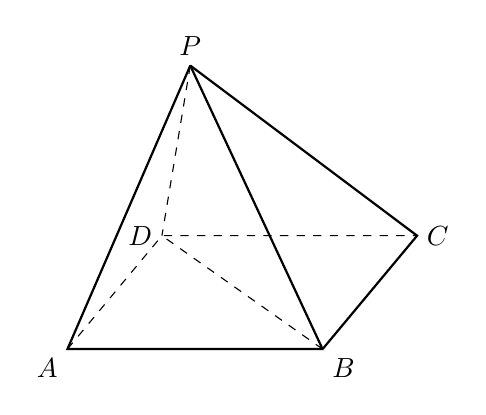
\begin{tikzpicture}[>=stealth,scale=1.2]
  % Coordinates
  \coordinate (A) at (-1.5,-0.8);
  \coordinate (B) at (1.2,-0.8);
  \coordinate (C) at (2.2,0.4);
  \coordinate (D) at (-0.5,0.4);
  \coordinate (P) at (-0.2,2.2);

  % Solid edges
  \draw[thick] (P) -- (A) -- (B) -- (C) -- (P);
  \draw[thick] (P) -- (B);

  % Dashed edges
  \draw[dashed] (A) -- (D) -- (C);
  \draw[dashed] (P) -- (D);
  \draw[dashed] (B) -- (D);

  % Labels
  \node[below left] at (A) {$A$};
  \node[below right] at (B) {$B$};
  \node[right] at (C) {$C$};
  \node[left] at (D) {$D$};
  \node[above] at (P) {$P$};
\end{tikzpicture}
\end{center}
\nopagebreak[4]
（1）求四棱锥 $P-ABCD$ 的体积；

（2）证明：$PA\perp BD$．

\Needspace{4\baselineskip}
\textbf{解析}

（1）在四棱锥 $P-ABCD$ 中，底面 $ABCD$ 为矩形，$AB=8$，$AD=4\sqrt{3}$。
侧面 $PAD$ 为等边三角形，其边长为 $AD=4\sqrt{3}$。
取 $AD$ 的中点为 $E$，连接 $PE$。
\Needspace{5\baselineskip}
在等边 $\triangle PAD$ 中，$PE\perp AD$，且
\nopagebreak[4]
\[
PE=\frac{\sqrt{3}}{2}AD=\frac{\sqrt{3}}{2}\times 4\sqrt{3}=6.
\]
过点 $P$ 作底面 $ABCD$ 的垂线，垂足为 $H$。
因为 $PE\perp AD$，$PH\perp\text{\text{底面} }ABCD$，由三垂线定理的逆定理可知 $EH\perp AD$。
所以 $\angle PEH$ 即为侧面 $PAD$ 与底面 $ABCD$ 所成二面角的平面角，
已知该二面角为 $60^\circ$，即 $\angle PEH=60^\circ$。
在 $\text{Rt}\triangle PHE$ 中：
\Needspace{5\baselineskip}
四棱锥的高为：
\nopagebreak[4]
\[
h=PH=PE\sin 60^\circ=6\times\frac{\sqrt{3}}{2}=3\sqrt{3}.
\]
\Needspace{5\baselineskip}
矩形底面 $ABCD$ 的面积为：
\nopagebreak[4]
\[
S_{ABCD}=AB\times AD=8\times 4\sqrt{3}=32\sqrt{3}.
\]
\Needspace{5\baselineskip}
因此，四棱锥 $P-ABCD$ 的体积为：
\nopagebreak[4]
\[
V=\frac{1}{3}S_{ABCD}\cdot h=\frac{1}{3}\times 32\sqrt{3}\times 3\sqrt{3}=96.
\]

\Needspace{5\baselineskip}
（2）在 $\text{Rt}\triangle PHE$ 中，
\nopagebreak[4]
\[
EH=PE\cos 60^\circ=6\times\frac{1}{2}=3.
\]
在底面矩形 $ABCD$ 中，$AB\perp AD$ 且 $EH\perp AD$，所以 $EH\parallel AB$。
因为侧面 $PAD$ 与底面所成二面角为锐角 $60^\circ$，垂足 $H$ 落在底面矩形内部。
以 $A$ 为原点，射线 $AD$ 为 $x$ 轴正半轴，射线 $AB$ 为 $y$ 轴正半轴，过 $A$ 点垂直于底面向上为 $z$ 轴正半轴建立空间直角坐标系。
\Needspace{5\baselineskip}
由题设各点坐标为：
\nopagebreak[4]
\[
A(0,0,0),\quad D(4\sqrt{3},0,0),\quad B(0,8,0),\quad C(4\sqrt{3},8,0).
\]
因为 $E$ 为 $AD$ 中点，所以 $E(2\sqrt{3},0,0)$。
点 $H$ 在底面内，满足 $EH\parallel AB$ 且 $EH=3$，故 $H(2\sqrt{3},3,0)$。
\Needspace{5\baselineskip}
因为 $PH\perp\text{\text{底面}}$ 且 $PH=3\sqrt{3}$，所以顶点 $P$ 的坐标为：
\nopagebreak[4]
\[
P(2\sqrt{3},3,3\sqrt{3}).
\]
\Needspace{5\baselineskip}
从而有向量：
\nopagebreak[4]
\[
\vec{PA}=\vec{OA}-\vec{OP}=(-2\sqrt{3},-3,-3\sqrt{3}),
\]
\nopagebreak[4]
\[
\vec{BD}=\vec{OD}-\vec{OB}=(4\sqrt{3},-8,0).
\]
\Needspace{5\baselineskip}
计算数量积：
\nopagebreak[4]
\[
\vec{PA}\cdot\vec{BD}=(-2\sqrt{3})\times(4\sqrt{3})+(-3)\times(-8)+(-3\sqrt{3})\times 0=-24+24+0=0.
\]
因为 $\vec{PA}\cdot\vec{BD}=0$，所以 $\vec{PA}\perp\vec{BD}$。
即 $PA\perp BD$。

\gkanswer{答案：（1）$96$；（2）证明见解析}

\end{answer}
\begin{answer}
\gksolhead{21}{}

\textbf{题目}：

（本小题满分 12 分）

双曲线 $\dfrac{x^2}{a^2}-\dfrac{y^2}{b^2}=1$（$a>1,b>0$）的焦点距为 $2c$，直线 $l$ 过点 $(a,0)$ 和 $(0,b)$，且点 $(1,0)$ 到直线 $l$ 的距离与点 $(-1,0)$ 到直线 $l$ 的距离之和 $s\geqslant\dfrac{4}{5}c$．求双曲线的离心率 $e$ 的取值范围．

\Needspace{4\baselineskip}
\textbf{解析}

双曲线的标准方程为 $\dfrac{x^2}{a^2}-\dfrac{y^2}{b^2}=1$（$a>1,b>0$），焦点距为 $2c$，则 $c^2=a^2+b^2$。
直线 $l$ 过点 $(a,0)$ 和 $(0,b)$，其截距式方程为 $\dfrac{x}{a}+\dfrac{y}{b}=1$，
\Needspace{5\baselineskip}
化为一般式方程为：
\nopagebreak[4]
\[
bx+ay-ab=0.
\]
由点到直线的距离公式：
\Needspace{5\baselineskip}
点 $(1,0)$ 到直线 $l$ 的距离为：
\nopagebreak[4]
\[
d_1=\frac{|b\cdot 1+a\cdot 0-ab|}{\sqrt{a^2+b^2}}=\frac{|b-ab|}{c}=\frac{b|1-a|}{c}.
\]
\Needspace{5\baselineskip}
因为 $a>1$，所以 $|1-a|=a-1$，即
\nopagebreak[4]
\[
d_1=\frac{b(a-1)}{c}.
\]
\Needspace{5\baselineskip}
点 $(-1,0)$ 到直线 $l$ 的距离为：
\nopagebreak[4]
\[
d_2=\frac{|b\cdot(-1)+a\cdot 0-ab|}{\sqrt{a^2+b^2}}=\frac{|-b-ab|}{c}=\frac{b(a+1)}{c}.
\]
\Needspace{5\baselineskip}
因此两点到直线 $l$ 的距离之和为：
\nopagebreak[4]
\[
s=d_1+d_2=\frac{b(a-1)+b(a+1)}{c}=\frac{2ab}{c}.
\]
\Needspace{5\baselineskip}
已知 $s\geqslant\dfrac{4}{5}c$，即
\nopagebreak[4]
\[
\frac{2ab}{c}\geqslant\frac{4}{5}c\implies ab\geqslant\frac{2}{5}c^2.
\]
\Needspace{5\baselineskip}
两边同除以 $c^2$：
\nopagebreak[4]
\[
\frac{a}{c}\cdot\frac{b}{c}\geqslant\frac{2}{5}.
\]
由双曲线离心率的定义 $e=\dfrac{c}{a}>1$，可得 $\dfrac{a}{c}=\dfrac{1}{e}$。
\Needspace{5\baselineskip}
又由 $b^2=c^2-a^2$，得：
\nopagebreak[4]
\[
\frac{b}{c}=\sqrt{1-\frac{a^2}{c^2}}=\sqrt{1-\frac{1}{e^2}}=\frac{\sqrt{e^2-1}}{e}.
\]
\Needspace{5\baselineskip}
将此代入不等式中：
\nopagebreak[4]
\[
\frac{1}{e}\cdot\frac{\sqrt{e^2-1}}{e}\geqslant\frac{2}{5}\implies\frac{\sqrt{e^2-1}}{e^2}\geqslant\frac{2}{5}.
\]
\Needspace{5\baselineskip}
因为 $e>1$，两边平方得：
\nopagebreak[4]
\[
\frac{e^2-1}{e^4}\geqslant\frac{4}{25}.
\]
\Needspace{5\baselineskip}
令 $t=e^2$（$t>1$），不等式化为：
\nopagebreak[4]
\[
\frac{t-1}{t^2}\geqslant\frac{4}{25}\implies 4t^2-25t+25\leqslant 0.
\]
\Needspace{5\baselineskip}
因式分解：
\nopagebreak[4]
\[
(4t-5)(t-5)\leqslant 0.
\]
\Needspace{5\baselineskip}
解得：
\nopagebreak[4]
\[
\frac{5}{4}\leqslant t\leqslant 5\implies\frac{5}{4}\leqslant e^2\leqslant 5.
\]
\Needspace{5\baselineskip}
因为 $e>1$，所以
\nopagebreak[4]
\[
\frac{\sqrt{5}}{2}\leqslant e\leqslant\sqrt{5}.
\]
因此，双曲线的离心率 $e$ 的取值范围是 $\left[\dfrac{\sqrt{5}}{2},\sqrt{5}\right]$。

\gkanswer{答案：$\left[\dfrac{\sqrt{5}}{2}, \sqrt{5}\right]$}

\end{answer}
\begin{answer}
\gksolhead{22}{}

\textbf{题目}：

（本小题满分 14 分）

已知函数 $f(x)=\mathrm{e}^{-x}(\cos x+\sin x)$，将满足 $f'(x)=0$ 的所有正数 $x$ 从小到大排成数列 $\{x_n\}$．

（1）证明数列 $\{f(x_n)\}$ 为等比数列；

（2）记 $S_n$ 是数列 $\{x_n f(x_n)\}$ 的前 $n$ 项和，求 $\lim\limits_{n\to\infty}\dfrac{S_1+S_2+\cdots+S_n}{n}$．

\Needspace{4\baselineskip}
\textbf{解析}

（1）函数为 $f(x)=\mathrm{e}^{-x}(\cos x+\sin x)$。
\Needspace{5\baselineskip}
对其求导：
\nopagebreak[4]
\[
\begin{aligned}
f'(x)&=(\mathrm{e}^{-x})'(\cos x+\sin x)+\mathrm{e}^{-x}(\cos x+\sin x)'\\
&=-\mathrm{e}^{-x}(\cos x+\sin x)+\mathrm{e}^{-x}(-\sin x+\cos x)\\
&=\mathrm{e}^{-x}(-\cos x-\sin x-\sin x+\cos x)\\
&=-2\mathrm{e}^{-x}\sin x.
\end{aligned}
\]
令 $f'(x)=0$。由于 $\mathrm{e}^{-x}>0$ 恒成立，所以必有 $\sin x=0$。
\Needspace{5\baselineskip}
因为 $x$ 为正数，满足条件的所有正数从小到大依次为：
\nopagebreak[4]
\[
x_n=n\pi\quad (n=1,2,3,\dots).
\]
\Needspace{5\baselineskip}
将 $x_n$ 代入原函数：
\nopagebreak[4]
\[
f(x_n)=\mathrm{e}^{-n\pi}(\cos n\pi+\sin n\pi).
\]
\Needspace{5\baselineskip}
因为对于正整数 $n$，$\sin n\pi=0$，$\cos n\pi=(-1)^n$，所以：
\nopagebreak[4]
\[
f(x_n)=\mathrm{e}^{-n\pi}(-1)^n=(-\mathrm{e}^{-\pi})^n.
\]
\Needspace{5\baselineskip}
计算相邻两项之比：
\nopagebreak[4]
\[
\frac{f(x_{n+1})}{f(x_n)}=\frac{(-\mathrm{e}^{-\pi})^{n+1}}{(-\mathrm{e}^{-\pi})^n}=-\mathrm{e}^{-\pi}.
\]
此比值为与 $n$ 无关的常数，且首项 $f(x_1)=-\mathrm{e}^{-\pi}\neq 0$。
因此数列 $\{f(x_n)\}$ 是以 $-\mathrm{e}^{-\pi}$ 为首项、$-\mathrm{e}^{-\pi}$ 为公比的等比数列。

\Needspace{5\baselineskip}
（2）由题意，数列 $\{x_n f(x_n)\}$ 的通项为：
\nopagebreak[4]
\[
u_n=x_n f(x_n)=n\pi(-\mathrm{e}^{-\pi})^n.
\]
记公比 $q=-\mathrm{e}^{-\pi}$。显然 $|q|=\mathrm{e}^{-\pi}=\dfrac{1}{\mathrm{e}^\pi}<1$。
前 $n$ 项和为 $S_n=\sum\limits_{k=1}^n u_k=\pi\sum\limits_{k=1}^n k q^k$。
令 $T_n=\sum\limits_{k=1}^n k q^k=q+2q^2+3q^3+\cdots+n q^n$。
\Needspace{5\baselineskip}
用错位相减法求和：
\nopagebreak[4]
\[
q T_n=q^2+2q^3+3q^4+\cdots+(n-1)q^n+n q^{n+1}.
\]
\Needspace{5\baselineskip}
两式相减得：
\nopagebreak[4]
\[
(1-q)T_n=q+q^2+q^3+\cdots+q^n-n q^{n+1}=\frac{q(1-q^n)}{1-q}-n q^{n+1}.
\]
\Needspace{5\baselineskip}
所以：
\nopagebreak[4]
\[
T_n=\frac{q(1-q^n)}{(1-q)^2}-\frac{n q^{n+1}}{1-q}.
\]
因为 $|q|<1$，当 $n\to\infty$ 时，$q^n\to 0$ 且 $n q^{n+1}\to 0$，
\Needspace{5\baselineskip}
因此：
\nopagebreak[4]
\[
\lim_{n\to\infty} T_n=\frac{q}{(1-q)^2}.
\]
\Needspace{5\baselineskip}
故：
\nopagebreak[4]
\[
\lim_{n\to\infty} S_n=\pi\lim_{n\to\infty} T_n=\frac{\pi q}{(1-q)^2}.
\]
设常数 $L=\lim\limits_{n\to\infty} S_n=\dfrac{\pi q}{(1-q)^2}$。
\Needspace{5\baselineskip}
由极限的算术平均值性质（若数列收敛于常数 $L$，则其前 $n$ 项算术平均值亦收敛于 $L$）：
\nopagebreak[4]
\[
\lim_{n\to\infty}\frac{S_1+S_2+\cdots+S_n}{n}=L.
\]
\Needspace{5\baselineskip}
将 $q=-\mathrm{e}^{-\pi}$ 代入 $L$ 中计算：
\nopagebreak[4]
\[
L=\frac{\pi(-\mathrm{e}^{-\pi})}{(1-(-\mathrm{e}^{-\pi}))^2}=-\frac{\pi\mathrm{e}^{-\pi}}{(1+\mathrm{e}^{-\pi})^2}=-\frac{\pi\mathrm{e}^\pi}{(\mathrm{e}^\pi+1)^2}.
\]
\Needspace{5\baselineskip}
因此：
\nopagebreak[4]
\[
\lim_{n\to\infty}\frac{S_1+S_2+\cdots+S_n}{n}=-\frac{\pi\mathrm{e}^\pi}{(\mathrm{e}^\pi+1)^2}.
\]

\gkanswer{答案：（1）证明见解析；（2）$-\dfrac{\pi\mathrm{e}^\pi}{(\mathrm{e}^\pi+1)^2}$（或 $-\dfrac{\pi\mathrm{e}^{-\pi}}{(1+\mathrm{e}^{-\pi})^2}$）}

\end{answer}